%% ===========================================================================
\section{Experimental setup}
\label{sec:setup}
%% ===========================================================================

\begin{figure}[pos=t]
\centering
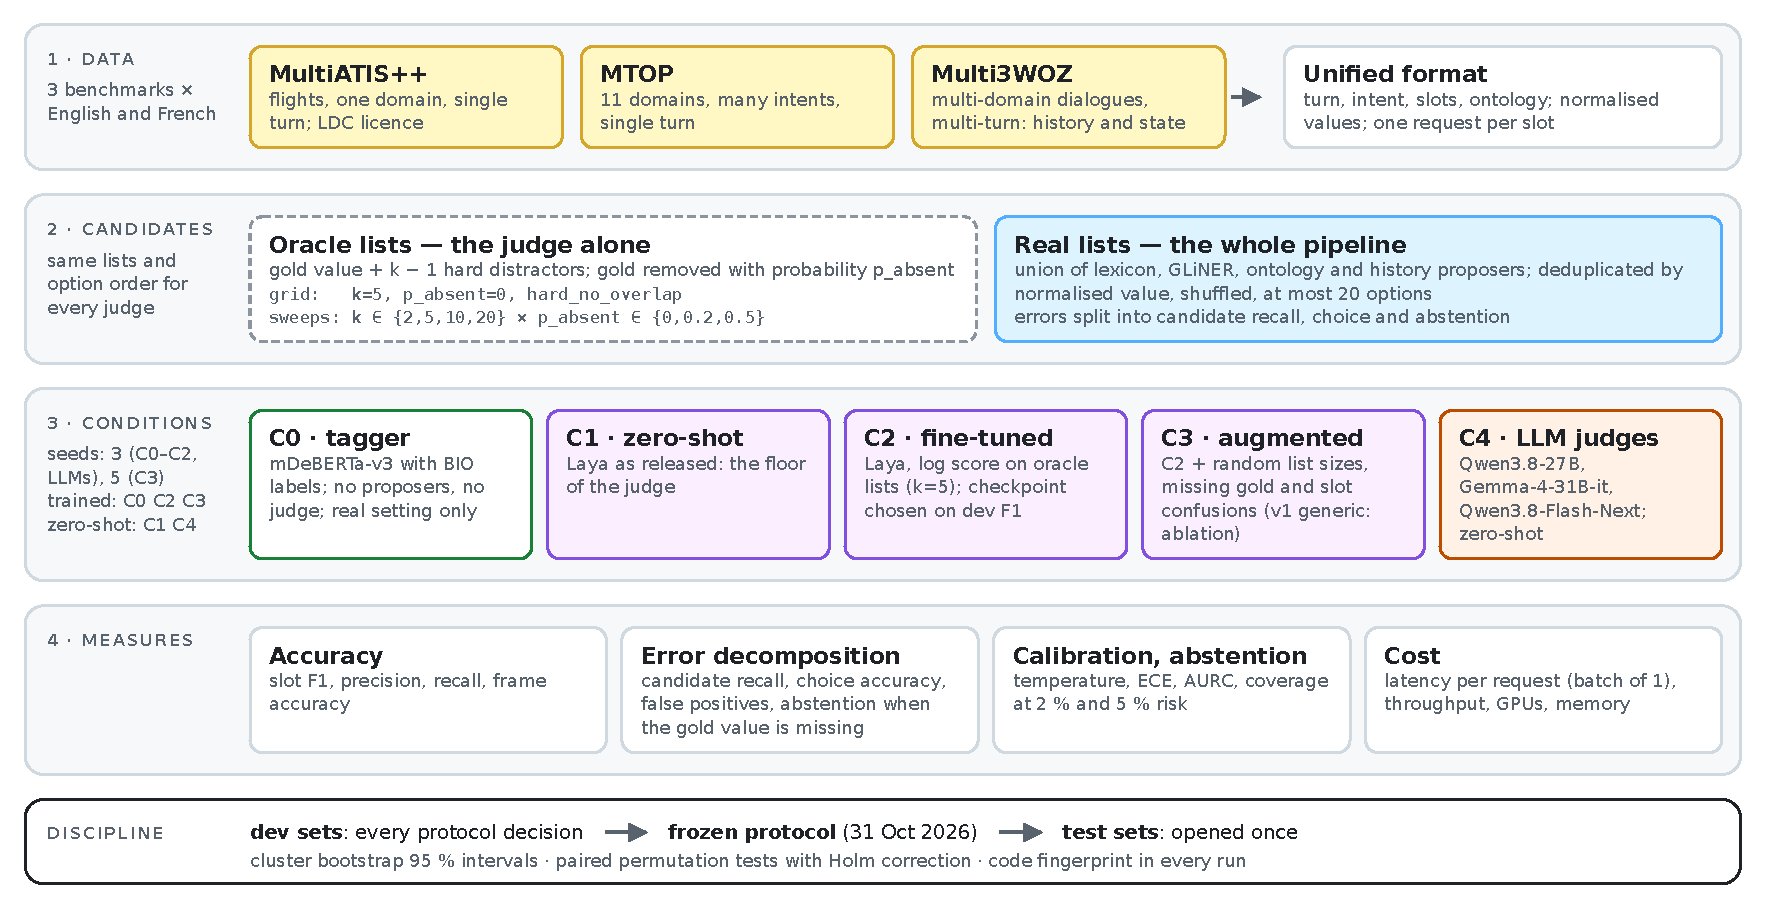
\includegraphics[width=\textwidth]{figures/protocol.pdf}
\caption{Experimental protocol. \textbf{(1)} Three span-annotated benchmarks, each in English and French, are converted to a unified format with one request per slot of the gold intent. \textbf{(2)} Every judge sees the same candidate lists in the same order: oracle lists isolate the judge (grid setting, and sweeps over the list size $k$ and the missing-gold rate $p_{\text{absent}}$), real lists from four proposers measure the whole pipeline. \textbf{(3)} Five conditions: a fine-tuned BIO tagger (C0), Laya zero-shot (C1), fine-tuned (C2) and fine-tuned with option-list augmentation (C3), and three open-weight LLM judges (C4). \textbf{(4)} Four families of measures: accuracy, error decomposition, calibration and selective decision, and cost. All protocol decisions were taken on development sets; the protocol was then frozen and each test set opened once.}
\label{fig:protocol}
\end{figure}

\subsection{Datasets and conversion}
\label{sec:datasets}

\Cref{fig:protocol} summarises the experimental design: the data, the two kinds of candidate lists, the compared conditions, the measures, and the separation between development and test data. The following subsections detail each part.

All three benchmarks annotate slots as text spans; we convert them to the candidate-selection format of \cref{sec:formulation} with a common schema and deterministic value normalisation (case, Unicode, numbers written in words, times, \cref{app:conversion}). Each converted split is written with a manifest that records the SHA-256 of the raw and produced files. \Cref{tab:datasets} summarises the data.

\begin{table}[pos=t]
\centering
\small
\caption{Datasets after conversion. Split sizes in utterances (MultiATIS++, MTOP) or dialogues (Multi3WOZ, one example per user turn). Request volumes are the number of (example, slot) requests submitted to the judge on the development split.}
\label{tab:datasets}
\begin{tabular}{@{}lllp{3.0cm}p{4.2cm}@{}}
\toprule
Dataset & Lang. & Turns & Train / dev / test & Dev requests \\
\midrule
MultiATIS++ & EN, FR & single & 4,478 / 500 / 893$^{a}$ & 30,310 per language (1,682 EN / 1,678 FR gold pairs) \\
MTOP & EN & single & 15,667 / 2,235 / 4,386 & 15,096 \\
     & FR & single & 11,814 / 1,577 / 3,193 & 9,832 \\
Multi3WOZ & EN, FR & multi & 7,440 / 860 / 860 dial. & 68,863 per language (7,708 gold pairs) \\
\bottomrule
\end{tabular}

\smallskip
\footnotesize $^{a}$ The LDC release provides only train (4,978) and test (893); we draw the development set from the training set (the 500 identifiers with the smallest SHA-256), aligned across languages. This is not the 4,488/490 split of the original paper.
\end{table}

\paragraph{MultiATIS++} \citep{xu2020multiatis,mansour2021atis7}: flight-information requests, one domain, with BIO labels. Spans are recovered as character offsets; for the rare multi-intent utterances (1--2\%), the first intent is the main intent. Slot descriptions were written once by hand (``fromloc.city\_name'' $\rightarrow$ ``departure city''), in English for English and in French for French, and frozen before evaluation. Thirteen lines of the French training split whose number of labels differs from the number of tokens are skipped.

\paragraph{MTOP} \citep{li2021mtop}: eleven domains and many intents (113 intents and 75 slots in English, 110 intents and 73 slots in French). We keep top-level slots; a nested slot becomes one top-level slot whose value is the full covered text, and its sub-tree is kept for a separate analysis. Slot descriptions were written by hand in English and used for both languages.

\paragraph{Multi3WOZ} \citep{hu2023multi3woz}: culturally adapted, multi-parallel versions of MultiWOZ dialogues, corrected release of 15 December 2023. One example is one user turn; its slots are the \emph{difference} between the dialogue state after and before the turn, the definition consistent with joint goal accuracy. We keep the five usual domains (hotel, train, restaurant, attraction, taxi; 30 slots). The history and the state before the turn are given to the judges. Multi3WOZ has no per-turn intent; we therefore query only the slots of the gold domain of the turn (\emph{domain filter}), which plays the role of the gold intent in the other datasets, and we pass the domain to the judge as a hint. Turns without a domain (15\%) are queried on all 30 slots. On 300 development turns, the filter reduces the number of requests from about 30 to 11 per turn, of which 12.6\% are expressed, and leaves out 8 of 420 gold pairs (1.9\%) that belong to another domain, which caps recall. The alternative of querying all 30 slots at every turn would quadruple the requests, 99\% of them unexpressed.

\paragraph{Requests} In all datasets, the judge receives the gold intent (or domain) and is asked about every slot that this intent allows. This isolates slot filling from intent classification; end-to-end evaluation with predicted intents is left for future work. About 94\% of the requests concern slots that are not expressed on MultiATIS++, which makes abstention a central part of the task.

\subsection{Conditions}
\label{sec:conditions}

\begin{table}[pos=t]
\centering
\small
\caption{Compared conditions. All judges see the same candidate lists and the same option order for a given seed.}
\label{tab:conditions}
\begin{tabular}{@{}lp{6.3cm}p{5.0cm}@{}}
\toprule
Code & Condition & Role \\
\midrule
C0 & Sequence tagger alone (mDeBERTa-v3-base, BIO labelling, fine-tuned) & classical extraction baseline (real setting only) \\
C1 & Laya zero-shot (published \texttt{multilingual} checkpoint) & floor of the judge \\
C2 & Laya fine-tuned, oracle lists $k=5$, $p_{\text{absent}}=0$ & effect of fine-tuning \\
C3 & Laya fine-tuned with confusion-oriented augmentation (v2) & robustness to list shape (RQ5) \\
C3 v1 & Laya fine-tuned with generic augmentation & ablation of the augmentation design \\
C4 & Open-weight LLM judges (three models), zero-shot & reference for the same role \\
\bottomrule
\end{tabular}
\end{table}

\Cref{tab:conditions} lists the conditions. Each judge is evaluated with oracle candidates (\texttt{hard\_no\_overlap}, $k=5$, $p_{\text{absent}}=0$: the \emph{grid setting}) and with real candidates. Sweeps over $k\in\{2,5,10,20\}$ and $p_{\text{absent}}\in\{0,0.2,0.5\}$, the \texttt{hard} distractor preset and the English-to-French transfer are analyses, run for the Laya judges on MultiATIS++ English. Few-shot LLM judges, a generative LLM extractor without proposers, the two-step judge mode (\cref{app:prompts}), unseen-domain splits and schema perturbations are left for future work (\cref{sec:limitations}).

\paragraph{The sequence tagger (C0)} C0 is the classical alternative to the proposer--judge architecture: a multilingual encoder, \texttt{microsoft/mdeberta-v3-base} (278\,M parameters; revision \texttt{a048466}, weights from the safetensors conversion \texttt{refs/pr/5}), fine-tuned to label every word of the current utterance with a BIO tag of the slots of the ontology (\texttt{B-}$\sigma$ for the first word of a value of slot $\sigma$, \texttt{I-}$\sigma$ for the following words of that value, \texttt{O} outside any value; in ``from New York to Paris'', \emph{New} is \texttt{B-from\_city}, \emph{York} is \texttt{I-from\_city} and \emph{Paris} is \texttt{B-to\_city}), in the spirit of JointBERT \citep{chen2019jointbert} but without an intent head (the gold intent is given to all conditions). Words are those of the candidate generators, and the label of a word is read on its first sub-word. Training labels come from the gold spans of the current utterance only, so that values taken from the history, the dialogue context or canonical forms that do not occur in the text cannot be learnt. The model is trained for 10 epochs with AdamW (learning rate $3\times10^{-5}$, batch 32, linear warm-up over 10\% of the steps), with three seeds, and the epoch with the best span F1 on the development set is kept. At inference, the decoded spans are normalised like the gold values; the best-scoring span of a slot is its only candidate, and C0 fills the slot with it, or answers ``not specified'' when the tagger proposes nothing. C0 therefore has no oracle setting.

\subsection{LLM judges and their configuration}
\label{sec:llms}

We selected recent open-weight models that fit the hardware and cover two families and two architectures (\cref{tab:llms}). All are served offline by vLLM~0.30.0 in text-only mode, with a context of 4,096 tokens, greedy decoding of one token and reasoning disabled. On 20 development examples (940 requests), the three models never produced a first token without an option letter. A fourth model from a third family, Mistral-Small-4-119B, could not be loaded by vLLM~0.30.0 (its text configuration declares no architecture) and was withdrawn; it may be added with a later vLLM version. A preliminary model (Qwen3-32B) used during development is not reported in the main results. The LLM judges are served with vLLM \citep{kwon2023vllm}, version 0.30.0.

\begin{table}[pos=t]
\centering
\small
\caption{Judges. Revisions are Hugging Face commit hashes (abbreviated); all are recorded in \texttt{MODELES.lock.json}.}
\label{tab:llms}
\resizebox{\textwidth}{!}{%
\begin{tabular}{@{}llllll@{}}
\toprule
Judge & Architecture & Parameters & Precision & GPUs & Revision \\
\midrule
Laya \texttt{multilingual} \citep{laya2026} & encoder, non-autoregressive & 0.32\,B (encoder) & fp32 (bf16 autocast) & 1 (shared) & \texttt{7b928d8} \\
Qwen3.8-27B \citep{qwen38} & dense decoder & 27.8\,B & BF16 & 1 & \texttt{1d4bf0f} \\
Gemma-4-31B-it \citep{gemma4report} & dense decoder & 31.3\,B & BF16 & 1 & \texttt{842da37} \\
Qwen3.8-Flash-Next-FP8 \citep{qwen38flashnext} & MoE (10 of 512 experts active) & 180\,B & FP8 & 2 & \texttt{236dfdf} \\
\bottomrule
\end{tabular}}
\end{table}

\subsection{Metrics}
\label{sec:metrics}

\paragraph{Accuracy} The main metric is the micro-averaged F1 over (slot, value) pairs, a ``not specified'' prediction not counting as a prediction, with precision and recall. \emph{Frame accuracy} is the share of examples whose whole set of slots is exactly right, with no extra slot; it makes the cost of false positives visible. Joint goal accuracy, the official Multi3WOZ metric, is not reported: our requests are restricted to the gold domain and evaluated turn by turn, which does not match the cumulative dialogue state it scores.

\paragraph{Decomposition} Because the F1 is dominated by abstention when most slots are unexpressed, we always report side by side: \emph{candidate recall} (share of gold pairs whose value is in the list), \emph{choice accuracy given present} (share of gold pairs correctly chosen when the value is in the list: the judge alone), the \emph{false-positive rate} (share of unexpressed requests for which a value is chosen), and the \emph{abstention rate when the gold value is absent} (share of requests with an expressed slot but no gold value in the list that are answered ``not specified'', the only answer that does not create an error).

\paragraph{Calibration and abstention} NLL, Brier score, ECE, temperature $T$, AURC, and coverage at 1\%, 2\% and 5\% risk (\cref{sec:decision}).

\paragraph{Cost} Latency per request (p50 and p95), throughput (requests per second), number of GPUs and memory. Accuracy runs are batched (Laya batches of 128 states, LLM batches of 256 prompts), and their latencies are batch-amortised. Latency proper is measured in separate runs with batches of size one (one request per call to the judge), on the first 100 development examples of each English dataset with oracle lists in the grid setting, seed 13, with nothing else running on the GPUs. For Laya, the first occurrence of each input length costs about 80\,ms, once (kernel selection for a new tensor shape); we report the p95 latency after this warm-up as well, since a deployed system would pad inputs to a few fixed lengths.

\subsection{Statistical protocol}
\label{sec:stats}

\paragraph{Seeds} Fine-tuned conditions use three seeds (C0, C2) or five (C3); the seed controls the training order, the subsampling of unexpressed requests and the oracle candidate draws. LLM judges are deterministic; their seeds only change the candidate draws (three in the final grid, one in the current development runs).

\paragraph{Intervals and tests} Confidence intervals (95\%) are percentile bootstrap intervals with 1,000 resamples of \emph{clusters} (dialogues for Multi3WOZ, utterances otherwise), never of isolated turns or requests. Each cluster is summarised by additive counts, and every metric is a ratio of sums with the same definitions as the point estimates. Paired comparisons use the clusters common to both systems: the difference and its interval come from a paired bootstrap, and the $p$-value from a permutation test that swaps the two systems cluster by cluster (10,000 permutations, two-sided). The Holm correction is applied over all comparisons and metrics of a family (stated with each result). With 10,000 permutations the smallest attainable $p$-value is $1/10{,}001$, so the smallest Holm-corrected value depends on the family size; we report such floor values as ``$p<10^{-4}$ before correction''.

\paragraph{Development and test discipline} All protocol decisions (distractor preset, checkpoint criterion, augmentation version, monolingual versus bilingual training, decision thresholds) were taken on development data. The protocol of the final runs (grid, seeds, analyses, families of tests, decision procedure) was then written down and frozen on 31 October 2026, together with the fingerprint of the code (\texttt{docs/protocole\_test.md} in the repository), and each test set was used in a single pass, from 31 October to 1 November 2026. During the early development phase, the MultiATIS++ English test split was opened several times; results obtained there are used only as exploratory evidence and are flagged as such (\cref{sec:threats}).

\subsection{Hardware, software and reproducibility}
\label{sec:repro}

All runs use one machine with two NVIDIA H200 NVL GPUs (143,771\,MiB each, driver 595.71.05, CUDA 13.0 runtime from Python wheels). Laya fits on a fraction of one GPU (peak memory 1.7\,GiB); the LLMs take one GPU (27--31\,B) or both (180\,B). The environment is locked with \texttt{uv} (Python 3.12.15, PyTorch 2.13.0, transformers 5.16.1, vLLM 0.30.0, laya 0.3.22, GLiNER 0.2.29); model revisions are pinned and runs are executed offline. Every run writes its resolved configuration, its predictions (one line per request, with the full probability vector) and its metrics, together with the hash of the configuration, the SHA-256 of the data manifests, and a fingerprint of all source and configuration files (\texttt{code\_sha256}), which does not depend on the version-control metadata of the machine. Reruns with the same seed give identical metrics, and repeated trainings give the same losses to the third decimal. \Cref{app:hyper} lists all hyperparameters.
